\documentclass[NET,english,aspectratio=169,notitleframe]{tumbeamer}

%settings
\usepackage[utf8]{inputenc}
\usepackage{pgfplotstable}
\usepackage{marvosym}
\usepackage{filecontents}
\usepackage{packages}
\usepackage{beamermods}

\usepackage[backend=bibtex, style=ieee]{biblatex}

\usepackage{csquotes}

\usetikzlibrary{calc}
\usetikzlibrary{arrows.meta}


% For lecture mode (use package option 'lecture'):
%\lecture[GRNVS]{Grundlagen Rechnernetze und Verteilte Systeme}
%\module{IN0010}
%\semester{SoSe\,2016}
%\assistants{Johannes Naab, Stephan Günther, Maurice Leclaire}

\usepackage{pgfplots}
\pgfplotsset{compat=newest}
\usepackage{tumcolor}
\usepackage{tumcolors}
\usepackage{textpos}


\usepackage{pgfpages}
\usepackage{ifthen}
% ============================================================================
% jobname solution
% ============================================================================
\newif\ifsolution%
\ifthenelse{\equal{\detokenize{notes}}{\jobname}}{%
\setbeameroption{show notes on second screen=bottom}
\setbeamercolor{note page}{bg=white, fg=black}
\setbeamercolor{note title}{bg=white!95!black, fg=black}
}{
}

%\xdefinecolor{orange}{cmyk}{0,0.65,0.95,0} 
%\xdefinecolor{dblue}{cmyk}{1,0.54,0.04,0.19}
%\xdefinecolor{blue}{cmyk}{1,0.43,0,0}  
%\xdefinecolor{lblue}{cmyk}{0.65,0.19,0.01,0.04}
%\xdefinecolor{green} {cmyk}{0.35,0,1,0.2} 
%xdefinecolor{yellow}{rgb}{1.00,0.71,0.00} 
%\colorlet{lgtorange}{orange!20} 
%\colorlet{lgtdblue}{dblue!20} 
%\colorlet{lgtblue}{blue!20} 
%\colorlet{lgtlblue}{lblue!20} 
%colorlet{lgtgreen}{green!20} 
%\colorlet{lgtyellow}{yellow!20}

\newcommand\Wider[2][3em]{%
\makebox[\linewidth][c]{%
  \begin{minipage}{\dimexpr\textwidth+#1\relax}
  \raggedright#2
  \end{minipage}%
  }%
}
\usepackage{cancel}
\usepackage{minted}


\addbibresource{lit.bib}


% For beamer mode (default):
 % jeder von dem wir hier irgendwas nehmen, alphabetisch sortiert
\author[Paul Emmerich, Simon Ellmann]{\textbf{Paul Emmerich}, \textbf{Simon Ellmann}, Fabian Bonk, Alex Egger, Thomas Günzel,\\ Stefan Huber,  Maximilian Pudelko, Maximilian Stadlmeier, Sebastian Voit}
\title{Safe and Secure Drivers in High-Level Languages}
\date{December 29, 2018}

\begin{document}

\setbeamertemplate{footline}{}
  \begin{frame}[c,noframenumbering]
%    \begin{tikzpicture}[overlay,remember picture]
%      \node[opacity=0.5,anchor=south east] at ($(current page.south east)+(-1,-1)$) {%
%    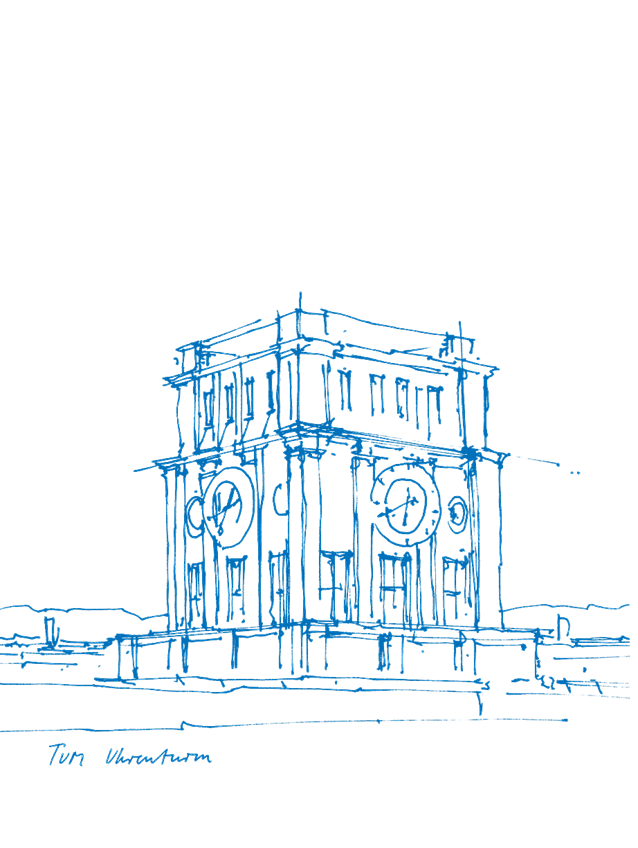
\includegraphics[width=.4\textwidth]{pics/TUM_Uhrenturm.png}};
%  \end{tikzpicture}
  \centering%
  \Large%
  \strut\textcolor{TUMBlue}{\inserttitle}%
  \\[4ex]%
  \normalsize%
  \strut\insertauthor%
  \\[2ex]%
  \footnotesize%
  \insertdate%
  \\[4ex]%
  \ifdefined\departmentname%
    \ifdefined\chairname%
      \chairname\\%
    \fi%
    \departmentname\\%
  \fi%
  \TUMname\\%
\end{frame}

  \begin{frame}[c,noframenumbering]
%    \begin{tikzpicture}[overlay,remember picture]
%      \node[opacity=0.5,anchor=south east] at ($(current page.south east)+(-1,-1)$) {%
%    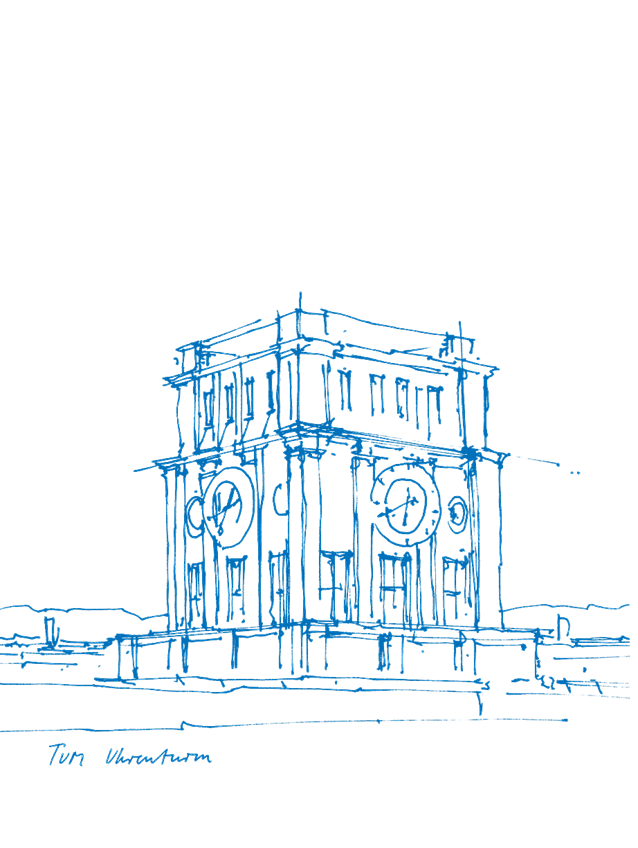
\includegraphics[width=.4\textwidth]{pics/TUM_Uhrenturm.png}};
%  \end{tikzpicture}
  \centering%
  \Large%
  \strut\textcolor{TUMBlue}{\inserttitle}%
  \\[4ex]%
  \normalsize%
  \strut{}\bfseries Paul Emmerich$^1$, Simon Ellmann$^2$, Fabian Bonk$^3$, Alex Egger$^4$, Thomas Günzel$^5$, Stefan Huber$^6$,  Maximilian Pudelko$^7$, Maximilian Stadlmeier$^8$, Sebastian Voit$^9$\normalfont %
  \\[2ex]%
  \footnotesize%
  $^1$C, thesis advisor\hspace{1em}
  $^2$Rust\hspace{1em}
  $^3$OCaml\hspace{1em}
  $^4$Haskell\hspace{1em}
  $^5$Swift\hspace{1em}
  $^6$IOMMU\hspace{1em}
  $^7$VirtIO driver\hspace{1em}
  $^8$C\#\hspace{1em}
  $^9$Go
  \\[4ex]%
    \ifdefined\departmentname%
    \ifdefined\chairname%
      \chairname\\%
    \fi%
    \departmentname\\%
  \fi%
  \TUMname\\%
\end{frame}
\setbeamertemplate{footline}[tumfootline]

\begin{frame}{About us}
% FIXME: use columns for images?
\begin{tikzpicture}[remember picture,overlay]
	\node[xshift=-2.5cm,yshift=-3cm] at (current page.north east) {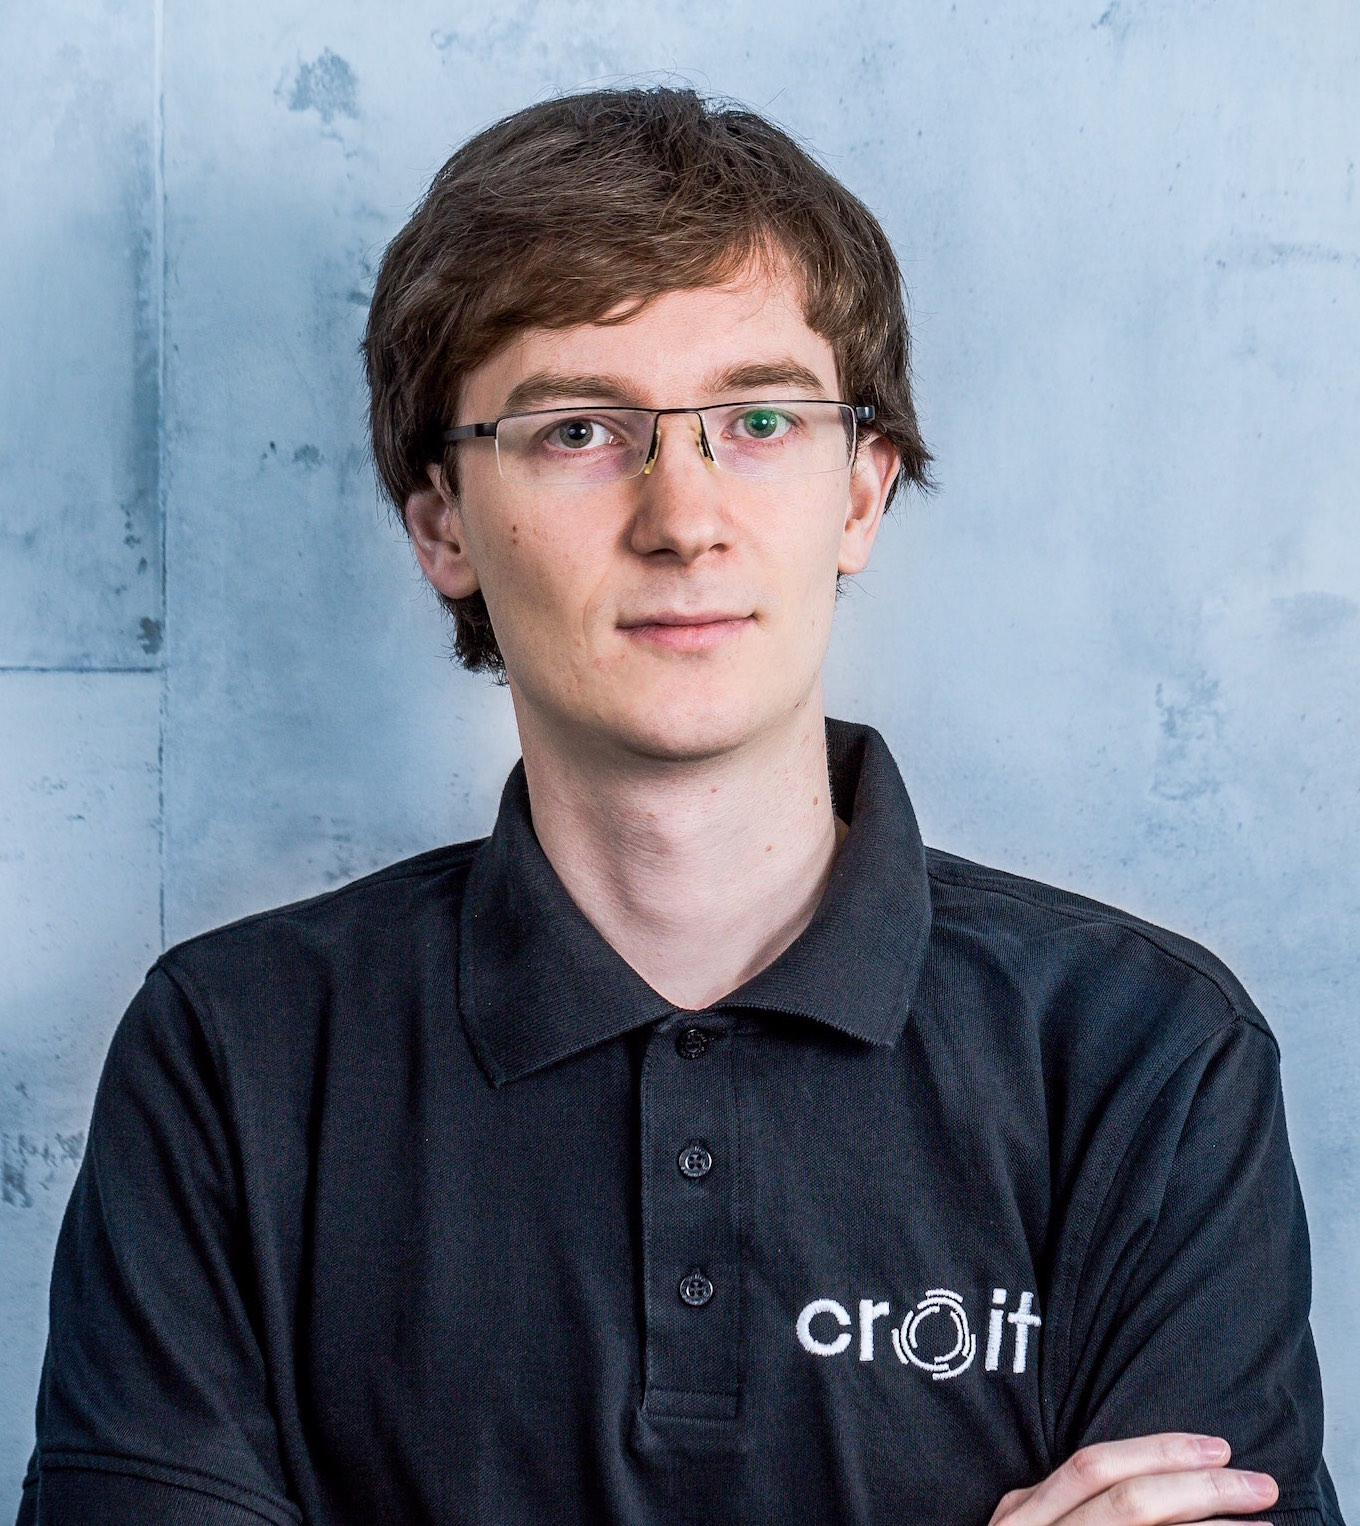
\includegraphics[width=0.2\textwidth]{pics/paul.jpg}};
%	\node[xshift=-2.5cm,yshift=-3cm] at (current page.south east) {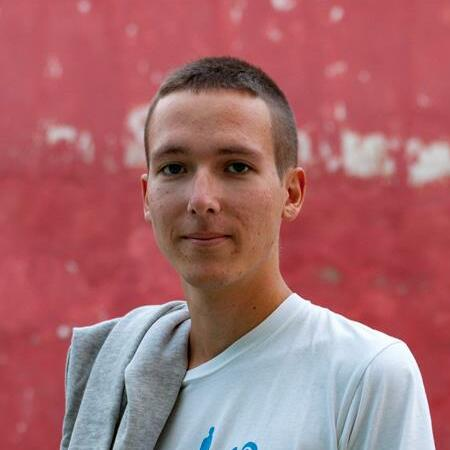
\includegraphics[width=0.2\textwidth]{pics/simon.jpg}};
\end{tikzpicture}
\emph{Paul}
\begin{itemize}
\item PhD student at Technical University of Munich
\item Researching performance of software packet processing systems
\end{itemize}
\vfill
\emph{Simon}
\begin{itemize}
\item HiWi/Research assistant
\item Rust driver as bachelor's thesis
\end{itemize}
\emph{Everyone else}
\begin{itemize}
\item Did a bachelor's thesis, master's thesis or other project with Paul as advisor
\end{itemize}
\end{frame}


\begin{frame}{Network drivers}
\centering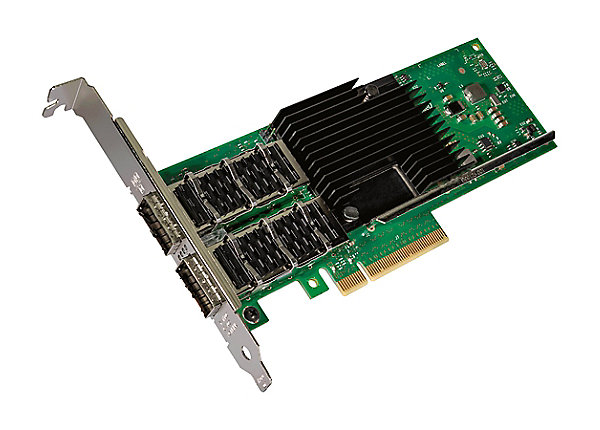
\includegraphics[width=0.66\textwidth]{pics/nic3}
\end{frame}

\begin{frame}{The ixy project}
\begin{itemize}
\item Attempt to write a simple yet fast user space network driver
\item It's a user space driver you can easily understand and read
\item $\approx$ 1,000 lines of C code, full of references to datasheets and specs
\item Supports Intel ixgbe NICs (82599, X540, Xeon D, ...)
\item New: supports VirtIO NICs (qemu/kvm and VirtualBox, we got a Vagrant setup!)
\item Check it out on GitHub: \url{https://github.com/emmericp/ixy}
\end{itemize}
\end{frame}


\begin{frame}{Expectation: Beautiful C code}
\begin{itemize}
\item Why write a driver in C?
\pause
\vspace{1em}
\item Most drivers are written in C
\item C is the lowest common denominator of systems programming languages
\item Everyone can read C?
\item C code can be beautiful
\end{itemize}
\end{frame}

\begin{frame}[fragile]{Reality: C can be ugly}
\begin{minted}[autogobble]{c}
#define mystery_macro(ptr, type, member) ({\
	const typeof(((type*)0)->member)* __mptr = (ptr);\
	(type*)((char*)__mptr - offsetof(type, member));\
})
\end{minted}
\end{frame}

\begin{frame}[fragile]{Reality: C can be ugly}
\begin{minted}[autogobble]{c}
#define container_of(ptr, type, member) ({\
	const typeof(((type*)0)->member)* __mptr = (ptr);\
	(type*)((char*)__mptr - offsetof(type, member));\
})
\end{minted}
\end{frame}


\begin{frame}[fragile]{Reality: C can be ugly}
\begin{minted}[autogobble]{c}
#define container_of(ptr, type, member) ({\
	const typeof(((type*)0)->member)* __mptr = (ptr);\
	(type*)((char*)__mptr - offsetof(type, member));\
})
\end{minted}
\begin{itemize}
\item Allows some ``inheritance'' in C to abstract driver implementations
\item Virtually all C drivers use this macro
\item The Linux kernel contains $\approx$ 15,000 uses of this macro
\end{itemize}
\end{frame}


%\setbeamertemplate{footline}{}
\begin{frame}{Reality: C can cause security problems}
%\centering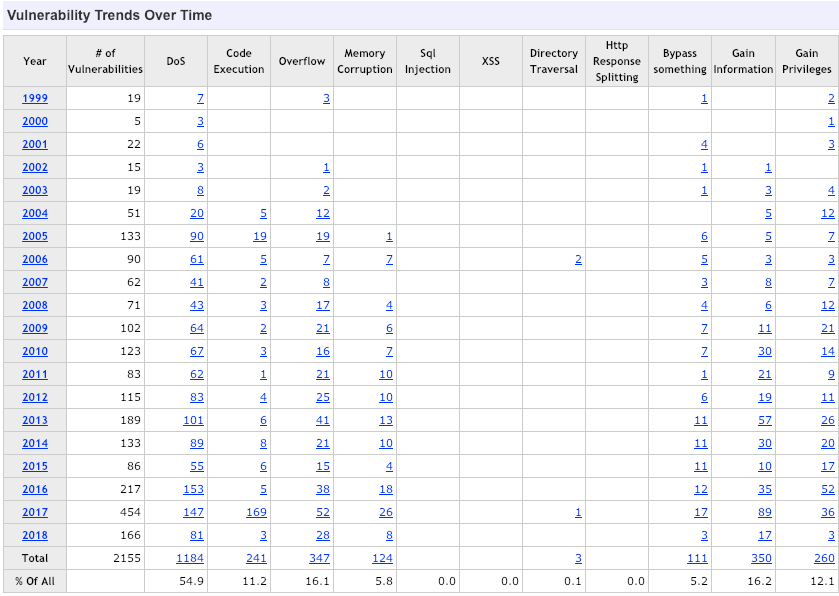
\includegraphics[width=0.65\textwidth]{pics/cve}\\
%\footnotesize bla subtitle
\begin{itemize}
\item blah biscuit paper \footnote{Biscuit}
\item ?? bugs
\item 40 due to memory safety
\vspace{1em}
\item How many of these are in drivers?
\pause
\item 39 are in drivers
\item (13 of these in Qualcomm WiFi driver)
\end{itemize}
\end{frame}
%\setbeamertemplate{footline}[tumfootline]

\begin{frame}{Should you really write new code in C in 2019?}
\begin{itemize}
\item If you have a choice: probably not, no
\pause
\item User space drivers can be written in \emph{any} language!
\item But are all languages an equally good choice?
\item Can high-level languages prevent bugs?
\item Is a JIT compiler or a garbage collector a problem in a driver?
\end{itemize}
\end{frame}

\setbeamertemplate{footline}{}
\begin{frame}{}
\centering
\includegraphics[width=0.65\textwidth]{pics/allthe1}
\end{frame}

\begin{frame}{}
\centering
\includegraphics[width=0.65\textwidth]{pics/allthe2}
\end{frame}

\begin{frame}{}
\centering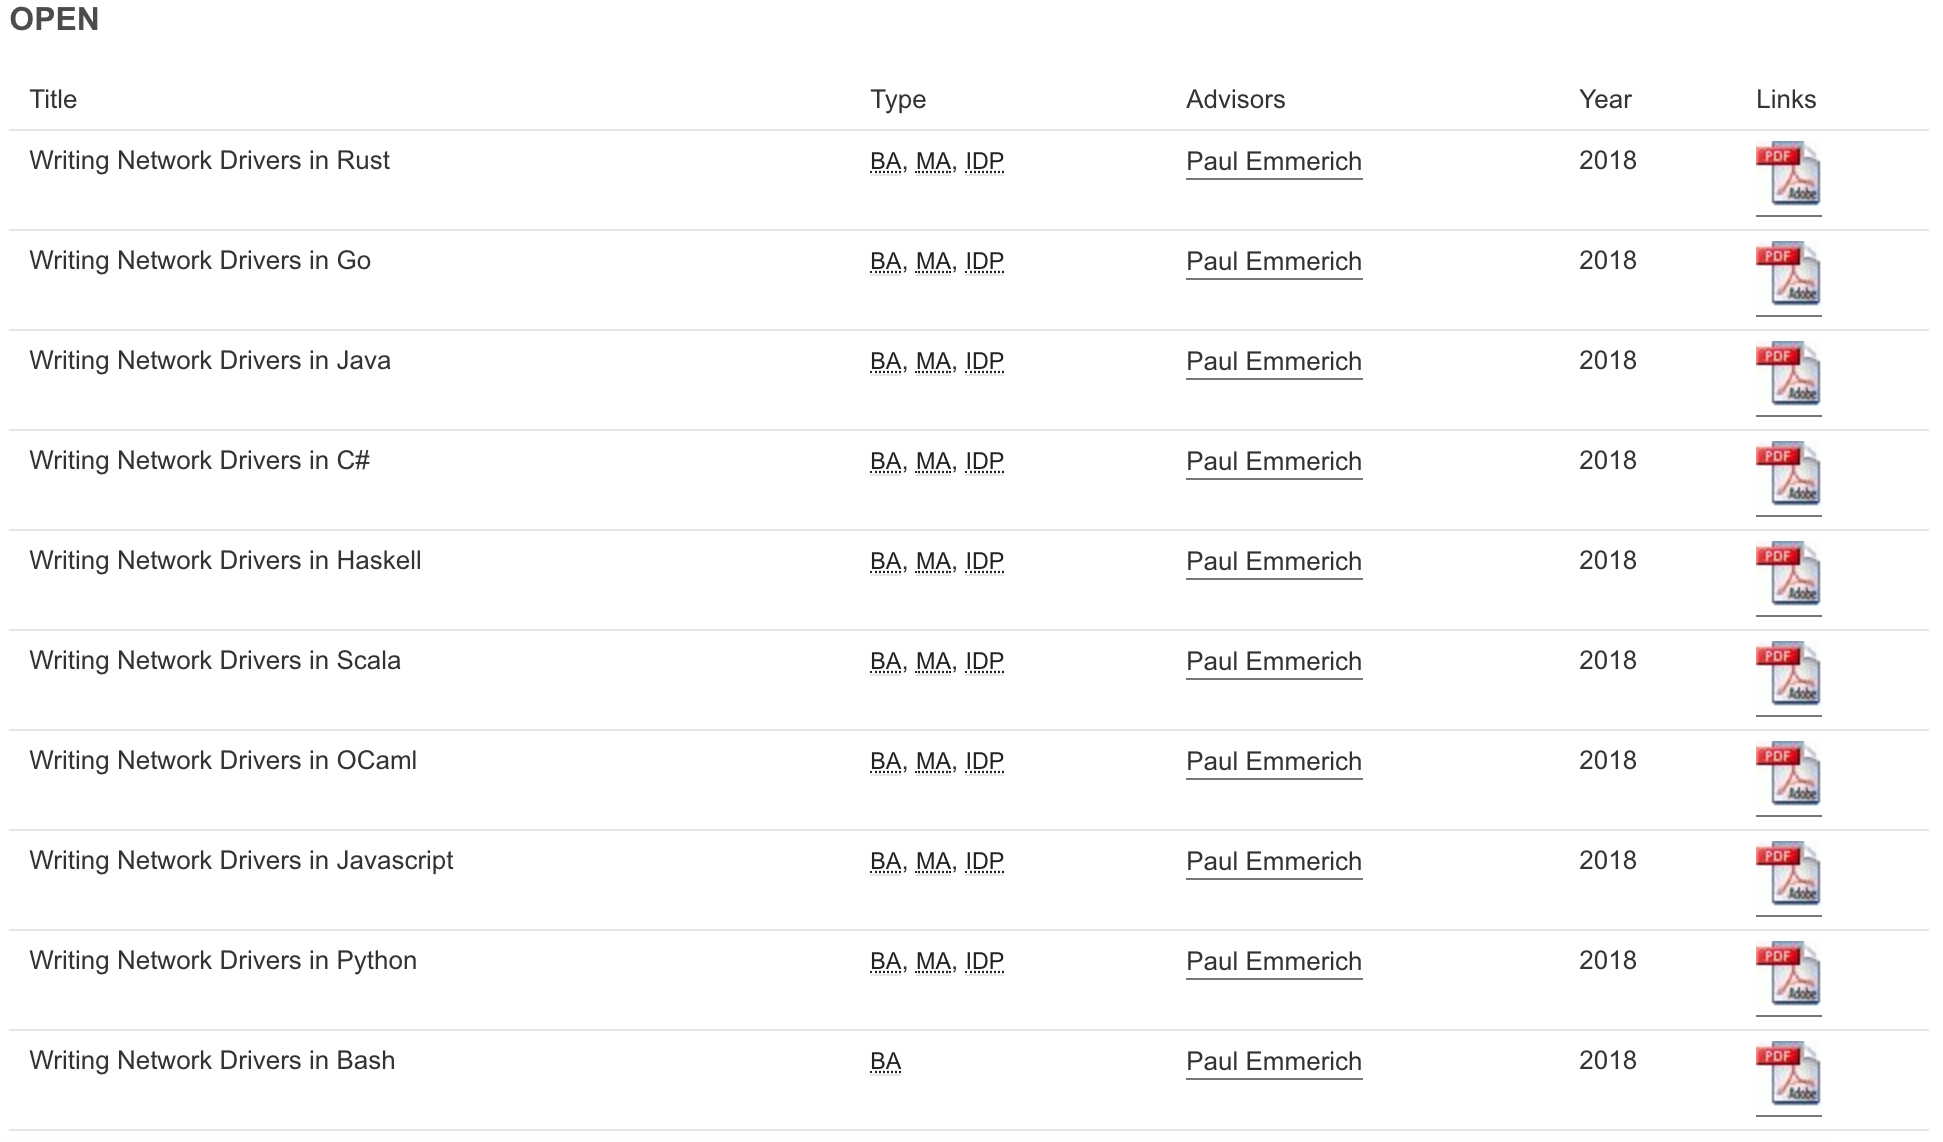
\includegraphics[width=0.85\textwidth]{pics/theses}
\end{frame}
\setbeamertemplate{footline}[tumfootline]


\begin{frame}{PCIe basics}
\begin{itemize}
\item MMIO
\item DMA
\item Interrupts
\end{itemize}
\end{frame}



\begin{frame}{How to write a user space driver in 4 simple steps}
\begin{itemize}
\item[1.] Unload kernel driver
\item[2.] \texttt{mmap} the PCIe MMIO address space
\item[3.] Figure out physical addresses for DMA
\item[4.] Write the driver
\end{itemize}
\end{frame}


\begin{frame}{Challenges for high-level languages}
\begin{itemize}
\item Access to \texttt{mmap} with the proper flags
\item Handle externally allocated memory in the language
\item Handle memory layouts/formats (i.e., access memory that looks like a given C struct)
\item Memory access semantics: memory barriers, volatile read/writes
\vspace{1em}
\pause
\item high-level unsafe blabla
\end{itemize}
\end{frame}



\begin{frame}{C\#}
\end{frame}

\begin{frame}{Swift}
\end{frame}

\begin{frame}{OCaml}
\end{frame}

\begin{frame}{Haskell}
\end{frame}

\begin{frame}{Go}
\end{frame}

\begin{frame}{Rust}
\end{frame}

\begin{frame}{Performance comparison}
\end{frame}

\begin{frame}{Garbage collection and JIT compilation vs. latency}
\end{frame}


\begin{frame}{Restricting devices with the IOMMU}
\end{frame}

\begin{frame}{Look ma, no root}
\end{frame}


\begin{frame}{Why to write a user space network driver?}
\end{frame}

\begin{frame}{(Maybe) network stack of the future}
\end{frame}

\begin{frame}{Why? Features!}
\end{frame}

\begin{frame}{Example: hardware timestamping}
\end{frame}


\begin{frame}{Conclusion: Check out our code}
%\centering \qrcode[height=3cm]{https://github.com/ixy-languages/ixy-languages}
\begin{itemize}
\item Meta-repository with links: \url{https://github.com/ixy-languages/ixy-languages}
\item Drivers are simple: don't be afraid of them
\item No kernel code needed :)
\end{itemize}
%\centering \Huge Q \& A
\end{frame}













\begin{frame}{What I care about}
\centering\begin{tikzpicture}[scale=1.35]
	\foreach \x in {1,2,...,7} {
		\pgfmathparse{40 - \x*5}\let\layershade\pgfmathresult
		\pgfmathparse{\x/2}\let\y\pgfmathresult
		\def\layercolor{TUMDarkerBlue}
		\draw[line width=.5pt,fill=\layercolor!\layershade]
			(0,\y) rectangle ($(4,\y+0.5)$);

	}
	\foreach \x in {1,2,...,7} {
		\node at (0.17,0.25+\x*0.5) {\fontsize{5}{6}\selectfont\bf \x};
	}
	\node at (2,0.75) {\fontsize{7}{8}\selectfont Physical};
	\node at (2,1.25) {\fontsize{7}{8}\selectfont Data Link};
	\node at (2,1.75) {\fontsize{7}{8}\selectfont Network};
	\node at (2,2.25) {\fontsize{7}{8}\selectfont \cancel{Transport}};
	\node at (2,2.75) {\fontsize{7}{8}\selectfont \cancel{Session}};
	\node at (2,3.25) {\fontsize{7}{8}\selectfont \cancel{Presentation}};
	\node at (2,3.75) {\fontsize{7}{8}\selectfont \cancel{Application}};
\end{tikzpicture}
\end{frame}


\begin{frame}{Not all apps run on top of HTTP}
Lots of network functionality is moving from specialized hardware to software:
\begin{itemize}
\item Routers
\item (Virtual) Switches
\item Firewalls
\item Middleboxes
\end{itemize}
Buzzwords: Network Function Virtualization, Service Function Chaining
\end{frame}

\begin{frame}{Example application}
%\centering\includestandalone{figures/softwarearch-simple}
\end{frame}


\begin{frame}{Normal applications}
%\centering\includestandalone{figures/softwarearch-classic}
\end{frame}

\begin{frame}{What it really looks like}
%\centering\includestandalone{figures/softwarearch-dragons}
\end{frame}

\begin{frame}{Performance}
\begin{itemize}
\item Packets per second on a 10\,Gbit/s link: up to \emph{14.88\,Mpps}
\item<2-> Packets per second on a 100\,Gbit/s link: up to \emph{148.8\,Mpps}
\item<3-> Clock cycles per packet on a 3\,GHz CPU with 14.88\,Mpps: $\approx 200$ cycles
\item<3-> Typical performance target: $\approx$ 5 to 10\,Mpps per CPU core for simple forwarding
\end{itemize}
\end{frame}

\begin{frame}{Performance: User space app}
\begin{itemize}
\item<1-> Typical performance target: $\approx$ 5 to 10\,Mpps per CPU core for simple forwarding
\item<1-> 5 to 10\,Mpps $=$ \emph{300 to 600 cycles} per packet at 3\,GHz
\vspace{1em}
\item<2-> Time to cross the user space boundary: very very long
\vspace{1em}
\item<3-> Single-core forwarding performance with sockets: $\approx$ 0.3\,Mpps
\item<3-> Single-core forwarding performance with libpcap: $\approx$ 1\,Mpps
%\item Latency of a typical hardware switch: $\le 1\,\mu s$
%\item Latency of a hardware switch: $\le 1\,\mu s$
\end{itemize}
\end{frame}

%\begin{frame}{Performance dragons?}
%\centering\includestandalone{figures/softwarearch-dragons}
%\end{frame}

\begin{frame}{Move the application into the kernel}
\centering\includestandalone{figures/softwarearch-kernel}
\end{frame}

\begin{frame}{Move the application into the kernel}
New problems:
\begin{itemize}
\item Cumbersome to develop
\item Usual kernel restrictions (e.g., C as programming language)
\item Application can (and will) crash the kernel
\end{itemize}
\end{frame}

\begin{frame}{Performance: Kernel app}
\begin{itemize}
\item<1-> Typical performance target: $\approx$ 5 to 10\,Mpps per CPU core for simple forwarding
\item<1-> 5 to 10\,Mpps $=$ \emph{300 to 600 cycles} per packet at 3\,GHz
\vspace{1em}
\item<2-> Time to receive a packet in the Linux kernel: $\approx \emph{500}$ \emph{cycles}
\item<3-> Time to send a packet in the Linux kernel: $\approx \emph{440}$ \emph{cycles}
\item<4-> Time to allocate, initialize, and free a \texttt{sk\_buff} in the Linux kernel: $\approx \emph{400}$ \emph{cycles}
\vspace{1em}
\item<5-> Single-core forwarding performance with Open vSwitch: $\approx$ 2\,Mpps
\item<5-> Hottest topic in the Linux kernel: XDP, which fixes some of these problems
\end{itemize}
\end{frame}


\begin{frame}{Do more in user space?}
%\centering\includestandalone{figures/softwarearch-moreuserspace}
\end{frame}

\begin{frame}{User space packet processing frameworks}
Examples for such frameworks
\begin{itemize}
\item netmap
\item PF\_RING ZC
\item pfq
\end{itemize}
\end{frame}

\begin{frame}{Problems}
\begin{itemize}
\item Non-standard API, custom kernel module required
\item Most frameworks require patched drivers
\item Exclusive access to the NIC for one application
\item No access to the usual kernel features
\begin{itemize}
\item Limited support for kernel integration in netmap
\end{itemize}
\item Poor support for hardware offloading features of NICs
\item Framework needs explicit support for each NIC, limited to a few NICs
\end{itemize}
\end{frame}

\begin{frame}{Do even more in user space?}
%\centering\includestandalone{figures/softwarearch-fulluserspace}
\end{frame}

\begin{frame}{User space driver frameworks}
Examples for such frameworks
\begin{itemize}
\item DPDK
\item Snabb
\end{itemize}
\end{frame}

\begin{frame}{Problems}
\begin{itemize}
\item Non-standard API
\item Exclusive access to the NIC for one application
\item Framework needs explicit support for each NIC model
\begin{itemize}
\item DPDK supports virtually all $\ge$ 10\,Gbit/s NICs
\end{itemize}
\item Limited support for interrupts
\begin{itemize}
\item Interrupts not considered useful at $\ge$ 0.1\,Mpps
\end{itemize}
\item No access to the usual kernel features
\end{itemize}
\end{frame}


\begin{frame}{Hardware: Intel \texttt{ixgbe} family (10\,Gbit/s)}
\begin{itemize}
\item \texttt{ixgbe} family: 82599ES (aka X520), X540, X550, Xeon D embedded NIC
\item Commonly found in servers or as on-board chips
\item Very good datasheet publicly available
%\vspace{1em}
\item Almost no logic hidden behind black-box firmware
%\item<2-> Black-box firmware contains almost no magic
%\item<2-> Drivers for many newer NICs often just exchanges messages with the firmware
%\item<2-> Here: all hardware features directly exposed to the driver
\end{itemize}
\end{frame}


\newmintinline[ccode]{c}{}
\newmintinline[bashcode]{c}{}

\begin{frame}[fragile=singleslide]{Find the device we want to use}
\begin{Verbatim}[commandchars=\\\{\}]
# lspci
03:00.0 Ethernet controller: Intel Corporation 82599ES 10-Gigabit SFI/SFP+ ...
03:00.1 Ethernet controller: Intel Corporation 82599ES 10-Gigabit SFI/SFP+ ...
\end{Verbatim}
\end{frame}

\begin{frame}[fragile=singleslide]{Find the device we want to use}
\begin{Verbatim}[commandchars=\\\{\}]
# lspci
\textbf{03:00.0} Ethernet controller: Intel Corporation 82599ES 10-Gigabit SFI/SFP+ ...
\textbf{03:00.1} Ethernet controller: Intel Corporation 82599ES 10-Gigabit SFI/SFP+ ...
\end{Verbatim}
\end{frame}

\begin{frame}[fragile=singleslide]{Unload the kernel driver}
\begin{minted}{bash}
echo 0000:03:00.1 > /sys/bus/pci/devices/0000:03:00.1/driver/unbind
\end{minted}
%\begin{itemize}
%\item \ccode{asdf hi}
%\item \ccode|asdf|
%\item \mintinline{c}{hi}
%\end{itemize}
\end{frame}

\begin{frame}[fragile=singleslide]{\texttt{mmap} the PCIe configuration address space from user space}
\begin{minted}[autogobble]{c}
	int fd = open("/sys/bus/pci/devices/0000:03:00.0/resource0", O_RDWR);
	struct stat stat;
	fstat(fd, &stat);
	uint8_t* registers = (uint8_t*) mmap(NULL, stat.st_size, PROT_READ | PROT_WRITE,
	                                     MAP_SHARED, fd, 0);
\end{minted}
\end{frame}



\end{document}

